%% main.tex --- Bucket Brigade workshop paper (v4 draft)
%%
%% v4 is a content revision: the phase-diagram grid expanded from 7 cells
%% (v3 preview) to 39 cells (Nash) / 37 cells (PPO sweep), and a fourth NE
%% class `mixed' emerged at 9 of the 37 PPO cells. v4 also adds a 4x-budget
%% PPO sweep on the no-convergence cells.
%%
%% Authored via anvil:pub. Compiles with pdflatex + bibtex against the
%% anvil-paper class shipped at .anvil/skills/pub/templates/anvil-paper.cls.
%% Figure 2 is rendered offline by figures/src/recalibrated_heatmap.py and
%% included as a PDF; it now reads from
%% experiments/p3_specialization/phase_diagram_ppo_v2/recalibrated_verdict.json
%% rather than the v3 phase_diagram_ppo location.

\documentclass{anvil-paper}

% Extra packages used by this paper specifically.
\usepackage{tikz}
\usetikzlibrary{patterns}
\usepackage{array}

\title{Bucket Brigade: A Parametric Cooperative-Competitive Benchmark with
Computable Nash Equilibrium Structure}
\author{Robb Walters \\ 2AM Logic}
\date{\today}

\begin{document}
\maketitle

\begin{abstract}
Canonical cooperative-MARL benchmarks (Overcooked, Hanabi, SMAC, Melting Pot,
MAgent, PettingZoo) trade equilibrium transparency for environment richness:
their state spaces are large enough that no Nash equilibrium is computable, so
when a new algorithm beats PPO on Overcooked the reader cannot tell whether
the algorithm has converged to the ``right'' joint policy or merely to a
Pareto-different one. \emph{Bucket Brigade} inverts this trade. It is a finite
parametric cooperative-competitive stochastic game on a ring of houses whose
per-agent action space at the minimal parameterization is~$8$, whose state
space is~$2304$ states, and whose three load-bearing scalars~$(\beta,\kappa,c)$
control equilibrium structure continuously across cells. We give the
environment specification, derive closed-form boundary inequalities for the
three Nash-equilibrium regimes (symmetric all-Work, asymmetric 1-Worker,
no-pure-NE collapse) via a single-house mean-field reduction, and report
empirical agreement between predicted and PPO-realised verdicts on a
$39$-cell phase diagram ($\beta{\times}\kappa{\times}c$). The reduction
correctly predicts the qualitative phase order
(collapse~$\to$~symmetric~$\to$~mixed~$\to$~asymmetric) and
$\beta$-independence; the $39$-cell grid surfaces a fourth empirical
class~--~\textsf{mixed} ($9/37$ PPO cells, both pure NE coexist)~--~which
the closed-form bound does not predict at the higher-$c$ regime where it
emerges. The trainability sweep ($37$ cells, $50$~iter${\times}2048$~steps,
$4$~seeds) recovers the same ordering under a per-cell NE-anchored metric:
$\texttt{gap\_closed\_ne}$ is largest on \textsf{symmetric\_only}~$(0.180)$,
smaller on \textsf{mixed}~$(0.107)$ and \textsf{asymmetric\_only}~$(0.059)$,
and negative on \textsf{no\_convergence}~$(-0.049)$. A
$4{\times}$-budget sweep on the no-convergence cells worsens
$\texttt{gap\_closed\_homogeneous}$ to~$-0.108$, indicating PPO's failure on
those cells is structural rather than budget-limited. The quantitative
$\kappa$-thresholds of the reduction disagree with the equilibrium solver
by $3$--$10\times$; we own this gap and attribute it to ring-locality,
per-agent ownership rewards, and the heuristic-strategy approximation. We position Bucket Brigade as a \emph{methodological
complement} to the surveyed benchmarks, not a replacement: it is the only
published parametric MARL game where the question ``did the algorithm
converge to the right equilibrium?'' admits a ground-truth answer.
\end{abstract}

\section{Introduction}
\label{sec:intro}

Multi-agent reinforcement learning evaluates new algorithms against benchmarks
whose Nash-equilibrium structure is not characterizable in closed form.
Overcooked-AI~\citep{overcooked2019}, DeepMind's Melting
Pot~\citep{meltingpot2021}, the Hanabi
Challenge~\citep{hanabi2020}, SMAC and SMACv2~\citep{smac2019,smacv2_2023},
MAgent~\citep{magent2018}, and the PettingZoo MPE
suite~\citep{pettingzoo2021} between them cover small cooperative
coordination, partial observability, scripted-opponent micromanagement, and
population-scale competition. None of them ship with a method that produces
the equilibrium strategy profile of the as-designed environment. When PPO
fails to learn a coordinated policy on Overcooked, the community is left to
debate whether the failure is the algorithm or the absence of a clean
attractor for self-play; neither hypothesis can be rejected because no oracle
exists for ``what should the learned policy look like.''

We introduce \emph{Bucket Brigade}, a finite parametric cooperative-competitive
stochastic game designed to invert this trade. At its minimal parameterization
the state space is $2304$~states and the per-agent action space is~$8$, so the
one-shot stage game is enumerable and standard equilibrium-computation tools
actually run. Across a smooth three-scalar parameter family~$(\beta,\kappa,c)$
the equilibrium structure transitions from symmetric all-Work to asymmetric
1-Worker (the textbook free-rider problem) to no-pure-NE collapse, with a
fourth empirically-observed regime~--~\textsf{mixed}, where both symmetric
and asymmetric pure NE coexist~--~appearing at high~$\kappa$ on the
higher-$c$ rows of the grid. The ground-truth target for each parameter cell
is known, so a failed PPO run is attributable to the algorithm rather than
to ambiguity about what convergence would mean. The pitch is exactly a
\emph{methodological complement} to the six canonical benchmarks above: those
exist for studying open-ended cooperation, generalization, and scale; Bucket
Brigade exists for studying equilibrium-convergence quality on a controlled
grid.

\paragraph{Contributions.} (1)~A self-contained formal specification of the
Bucket Brigade game~(\S\ref{sec:env}), recovering Volunteer's Dilemma, the
$N$-player Public Goods game, and Stag Hunt as named limits.
(2)~Closed-form boundary inequalities~(\S\ref{sec:ne}) for the three NE
regimes via a single-house mean-field reduction, together with an explicit
accounting of where the closed-form thresholds disagree with empirics and
where a fourth (\textsf{mixed}) class emerges that the bound does not
predict. (3)~A protocol, a per-cell NE-anchored evaluation metric, and the
first empirical results~(\S\ref{sec:trainability}) testing PPO trainability
against the NE phase diagram on the full~$39$-cell grid. The PPO ordering
recovered by the per-cell metric matches the analytical prediction
\textsf{symmetric}~$>$~\textsf{mixed}~$>$~\textsf{asymmetric}~$>$~%
\textsf{collapse}; a separate~$4{\times}$-budget sweep on the no-convergence
cells worsens, not improves, gap-closure~--~PPO's failure on those cells is
structural, not budget-limited. (4)~An honest positioning~(\S\ref{sec:related},%
~\S\ref{sec:discussion}) against the canonical benchmarks: Bucket Brigade is
small and artificial by design, and is not a substitute for any of them.
Throughout, we treat the analytical NE characterization as ground truth and
the PPO trainability sweep as a falsification test, in that order.

\section{The Bucket Brigade environment}
\label{sec:env}

\paragraph{Players and topology.}
A finite set of agents $\mathcal{I}{=}\{1,\ldots,N\}$ inhabits a cycle graph
$\mathcal{H}{=}\mathbb{Z}/H\mathbb{Z}$ of $H$ houses with neighbour edges. Each
house has status $h_h\in\{\textsc{Safe},\textsc{Burning},\textsc{Ruined}\}$;
\textsc{Ruined} is absorbing. The default ``10-house'' scenario fixes
$H{=}10,N{=}4,T_{\min}{=}12$; the minimal scenario fixes $H{=}2,N{=}4$.

\paragraph{Action and observation.}
Each agent $i$ chooses
$a_{t,i}{=}(a^{\text{house}},a^{\text{mode}},a^{\text{sig}})\in
\mathcal{H}\times\{0,1\}\times\{0,1\}$: a target house, a
\textsc{Work}/\textsc{Rest} bit, and a one-bit broadcast signal observable to
all agents on the next night. Per-agent action cardinality is $4H$ ($8$ at
$H{=}2$; $40$ at $H{=}10$). Joint-action cardinality at the minimal
parameterization is $8^4{=}4096$. Observation is symmetric perfect monitoring
with one-step signal delay: every agent observes the full state plus the
previous joint $(\ell_{t-1},\alpha_{t-1},\zeta_{t-1})$. There is no partial
observability of houses or agent positions; the signal channel is
non-binding cheap talk.

\paragraph{Transition dynamics.}
A single night consists of seven sequential phases applied in a fixed,
load-bearing order: (1)~signal write, (2)~location/mode write,
(3)~extinguish, (4)~burn-out, (5)~spread, (6)~spontaneous ignition,
(7)~reward and termination check. In the extinguish phase, if $w_h(a)$
agents \textsc{Work} at a \textsc{Burning} house, the house transitions to
\textsc{Safe} with probability $1-(1-\kappa)^{w_h(a)}$ (independent-workers
model). Every \textsc{Burning} house that survives the extinguish phase
transitions deterministically to \textsc{Ruined} in the burn-out phase. The
spread phase then ignites \textsc{Safe} neighbours of \textsc{Burning}
houses with probability $\beta$ per edge; under the canonical order, the
burn-out phase has already cleared all \textsc{Burning} sources, so spread is
inert in the within-night dynamics and contagion enters only via the
spontaneous-ignition phase~6 at rate $\rho$. (A contagion-active variant
that swaps phases 4 and 5 is available; the phase-diagram analysis below
uses the canonical order.)

\paragraph{Reward structure.}
The per-agent reward decomposes into three independently-parameterised terms:
a private work/rest cost ($-c$ for \textsc{Work}, $+c_{\text{rest}}{=}0.5$
for \textsc{Rest}; the free-rider gradient is the $c{+}c_{\text{rest}}$
asymmetry), a per-house ownership term ($r_{\text{own}}$ paid on save,
$p_{\text{own}}$ recurring on every \textsc{Ruined} night), and a team
welfare term proportional to the fraction of \textsc{Safe} and
\textsc{Ruined} houses. Ownership is assigned round-robin
($\text{owner}(h){=}h\bmod N$). The asymmetric reward variants in the
calibrated family let $r_{\text{own}},r_{\text{other}},p_{\text{own}},
p_{\text{other}}$ be set per-agent, breaking exchangeability.

\paragraph{Relationship to canonical templates.}
Bucket Brigade recovers, as named limits or restrictions, several textbook
templates: the $N$-player Volunteer's Dilemma at $H{=}1$; the $N$-player
Public Goods game when ownership weights collapse to uniform; Stag Hunt in
the $\kappa{\to}1$ limit; and a free-rider problem at the parameter cells
where the only NE is asymmetric (the ``rest-trap''). Formal proofs and a
complete notation table are deferred to the env-spec memo~\citep{bbenvspec};
\S\ref{sec:env} above is the minimal contract a reader needs to follow
\S\ref{sec:ne}.

\section{Equilibrium structure: closed-form boundaries}
\label{sec:ne}

The central contribution of this paper is a closed-form characterisation of
which Nash-equilibrium structure appears as a function of $(\beta,\kappa,c)$
in the 4-agent game. We derive it via a single-house mean-field reduction
that collapses the $H{=}10$ ring to a representative single house with all
$N{=}4$ agents present, absorbs multi-step contagion and ignition dynamics
into a per-night survival coefficient, and reads off the NE candidates as
algebraic inequalities.

\paragraph{Reduction.}
Fix the \texttt{minimal\_specialization} reward tuple
$W{=}(R_{\text{team}},P_{\text{team}},r_{\text{own}},r_{\text{other}},
p_{\text{own}},p_{\text{other}}){=}(10,10,50,0,100,0)$ and $\rho{=}0.02,
T_{\min}{=}12$. With $k$ workers at the house on a given night, the per-night
ruin probability for an initially-\textsc{Safe} house is
$q(k){=}\rho(1-\kappa)^k$ (under the canonical phase order, where $\beta$
does not enter the leading-order single-night payoff). Integrating the lost
per-house reward stream over $T_{\min}{=}12$ nights and collecting terms
yields
\[
  \mathbb{E}[\text{per-house reward loss}\mid k] = A\cdot\rho\cdot(1-\kappa)^k,
\]
with $A{=}r_{\text{own}}T_{\min}+p_{\text{own}}T_{\min}+P_{\text{team}}
T_{\min}/H{=}1812$ and survival coefficient
$\tilde A{:=}A\rho{=}36.24$. The marginal benefit of adding the $k$-th
worker is $\Delta(k){=}\tilde A\cdot\kappa\cdot(1-\kappa)^k$.

\paragraph{The three NE candidates.}
Writing $c_{\text{gap}}{:=}c+c_{\text{rest}}$ (so $c_{\text{gap}}{=}1.0$ when
the driver sets $c{=}0.5$), the deviation comparisons against the per-night
stage game under stationary opponent policies yield three inequalities.

The \emph{symmetric all-Work} NE exists iff a unilateral deviation from
$k{=}4$ to $k_{-i}{=}3$ does not pay:
\begin{equation}
  \tilde A\cdot\kappa\cdot(1-\kappa)^{3}\;\geq\;c_{\text{gap}}.
  \tag{S}\label{eq:S}
\end{equation}

The \emph{asymmetric 1-Worker} NE exists iff the lone worker prefers
\textsc{Work} ($k_{-i}{=}0$ deviation) and each free-rider prefers
\textsc{Rest} ($k_{-i}{=}1$ deviation):
\begin{equation}
  \tilde A\cdot\kappa\;\geq\;c_{\text{gap}}
  \quad\text{AND}\quad
  \tilde A\cdot\kappa\cdot(1-\kappa)\;<\;c_{\text{gap}}.
  \tag{A}\label{eq:A}
\end{equation}

The \emph{no-pure-NE collapse} regime holds whenever even a lone worker
cannot recover their cost, so neither~\eqref{eq:S} nor~\eqref{eq:A} can be
satisfied:
\begin{equation}
  \tilde A\cdot\kappa\;<\;c_{\text{gap}}.
  \tag{C}\label{eq:C}
\end{equation}

\paragraph{Predicted thresholds.}
Substituting $\tilde A{=}36.24,c_{\text{gap}}{=}1.0$ into~\eqref{eq:S}--%
\eqref{eq:C}: the collapse boundary~\eqref{eq:C} sits at
$\kappa\approx 0.028$; the symmetric NE exists on
$\kappa\in[0.030,0.65]$ via~\eqref{eq:S}; the asymmetric NE exists for
$\kappa\gtrsim 0.972$ via~\eqref{eq:A}. The qualitative phase order
$\kappa$-small$\to$$\kappa$-large is
\textsf{collapse}~$\to$~\textsf{symmetric\_only}~$\to$~\textsf{mixed}~$\to$~%
\textsf{asymmetric\_only}, and the derivation is structurally
$\beta$-independent under the canonical phase order.

\paragraph{Predicted vs.\ observed thresholds.}
The empirical phase diagram, computed by a heterogeneous Double-Oracle
solver over continuous heuristic-parameter strategies on a $39$-cell grid
($\beta\in\{0.1,0.5,0.9\}\times\kappa\in\{0.1,0.3,0.5,0.7,0.9\}\times
c\in\{0.5,1.0,2.0\}$, less six cells in the high-$\kappa\times c{=}0.5$
corner subsumed by the $c{=}1.0$ row; Figure~\ref{fig:phase}), recovers the
qualitative phase order and approximate $\beta$-independence at verdict
level: 12 of the 13 $(\kappa,c)$ rows with $\geq 2$ $\beta$ samples
show an identical verdict across all sampled $\beta$. The single
splitting row is $(\kappa{=}0.9, c{=}0.5)$, where $\beta{=}0.1$
yields \textsf{mixed} while $\beta\in\{0.5, 0.9\}$ yield
\textsf{asymmetric\_only}---a small but real anomaly we return to in
\S\ref{sec:discussion}. The grid surfaces \emph{four}
empirical classes: in addition to \textsf{symmetric\_only}~($n{=}12$),
\textsf{asymmetric\_only}~($n{=}11$), and \textsf{no\_convergence}~($n{=}6$),
a \textsf{mixed} class~($n{=}10$) appears in which the solver returns both
symmetric all-Work and asymmetric 1-Worker profiles as un-deviable,
primarily at $\kappa{=}0.9$ on the $c{\geq}1$ rows and at $\kappa{=}0.5,
c{=}2.0$. The closed-form bound~\eqref{eq:S}--\eqref{eq:C} does not predict
this fourth class at the higher-$c$ regime where it emerges: the derivation
pivots on $\tilde A\kappa(1-\kappa)^{k}$ being above or below
$c_{\text{gap}}$, which excludes the simultaneous-existence pattern.
Tightening the reduction to predict the \textsf{mixed} boundary in closed
form is in scope for future work.

The \emph{quantitative} $\kappa$-thresholds also disagree: the empirical
collapse boundary sits near $\kappa\approx 0.1$--$0.3$
(3--10$\times$ above the predicted~$0.028$), and the empirical asymmetric-NE
onset sits near $\kappa\approx 0.7$ (below the predicted~$0.972$). The
derivation gets the phase order right on the $39$-cell grid but the
thresholds wrong by $3$--$10\times$, the same gap we owned at the 7-cell
preview.

We \emph{own} this gap. The mean-field reduction has three identifiable
systematic biases. (i)~\emph{Ring locality}: the derivation puts all four
agents at one house, but empirically four agents distribute across ten
houses, so the effective per-house defence is $1{-}(1{-}\kappa)^{0.4}$ rather
than $1{-}(1{-}\kappa)^4$---roughly a $4\times$ weaker defence at $\kappa{=}0.5$,
which shifts the collapse boundary substantially upward into the
empirically-observed range $\kappa\in[0.1,0.3]$. (ii)~\emph{Per-agent
ownership rewards}: the analytical $A$ coefficient lumps $r_{\text{own}}$
and $p_{\text{own}}$ into the survival term, but the per-agent ownership
reward only fires on the agent's own house, scaling the off-own-house
contribution down by a factor of roughly $1/H$. (iii)~\emph{Heuristic
strategy space}: the empirical solver's ``free-riders'' are
\texttt{Firefighter} agents at \texttt{work\_tendency}${=}0.9$, not literal
\textsc{Rest} agents, so the effective $k_{-i}$ in the lone-worker's
deviation comparison is closer to $3.7$ than to~$1$. None of these
corrections are derivable in closed form without losing the algebraic
tractability that motivated the reduction; the natural extensions are
named in \S\ref{sec:discussion}.

\paragraph{Headline finding.}
The mean-field reduction correctly predicts \emph{three} structural
properties of the empirical phase diagram---the qualitative phase order,
$\beta$-independence under the canonical phase order, and the existence of a
no-pure-NE collapse regime at small~$\kappa$---none of which would be
derivable without the closed-form derivation. The quantitative
$\kappa$-thresholds are off by $3$--$10\times$, and a fourth empirical class
(\textsf{mixed}) appears at the higher-$c$ rows that the closed-form bound
does not predict; we report both as the paper's claim, not as weaknesses to
hide. The qualitative phase order furthermore transfers to the PPO
trainability sweep under a per-cell NE-anchored metric
(\S\ref{sec:trainability}). The per-cell predicted-vs-empirical table and
the full bias accounting appear in~\citep{bbnestructure}.

\begin{figure}[t]
  \centering
  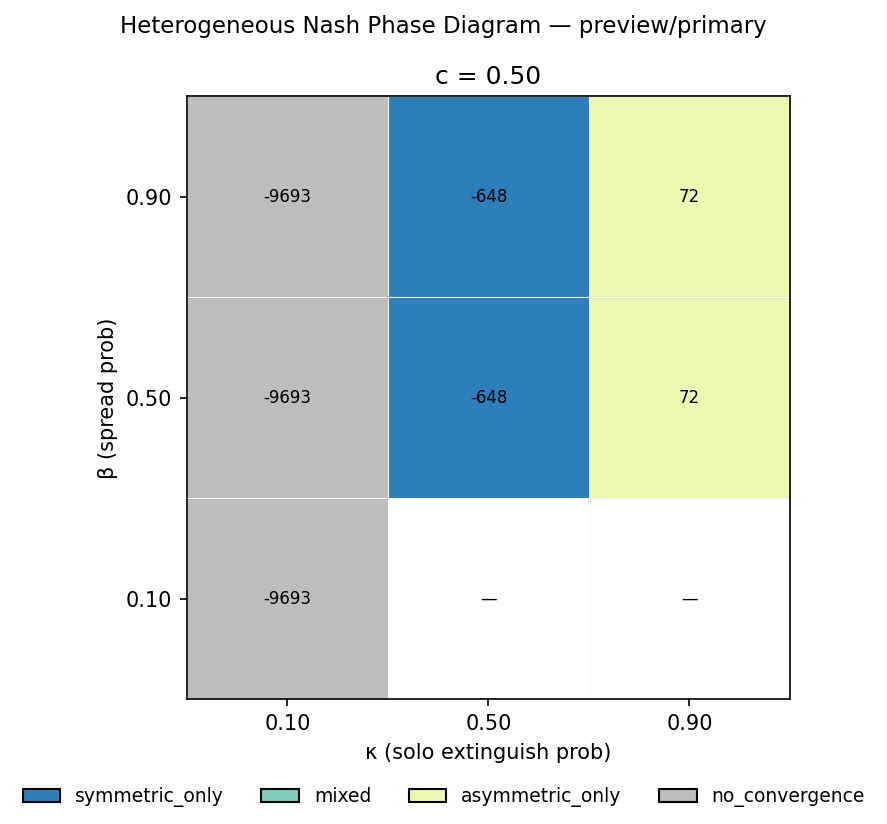
\includegraphics[width=0.92\linewidth]{figures/phase_diagram.png}
  \caption{Empirical NE phase diagram for 4-agent Bucket Brigade across
  $(\beta,\kappa)$ at $c{=}0.5,\rho{=}0.02,T_{\min}{=}12$ under the
  \texttt{minimal\_specialization} reward tuple. Each cell is the verdict of
  a heterogeneous Double-Oracle solver over the continuous
  heuristic-parameter strategy space (Hero, Firefighter, FreeRider, $\ldots$).
  The figure shows the $c{=}0.5$ panel of the full~$39$-cell grid that adds
  $c\in\{1.0,2.0\}$ panels and intermediate $\kappa\in\{0.3,0.7\}$ rows;
  see~\citep{bbnestructure} for the full grid. Four regimes appear across
  the grid: \textsf{no\_convergence} at low~$\kappa$ (collapse),
  \textsf{symmetric\_only} at moderate~$\kappa$ (Hero NE dominates),
  \textsf{asymmetric\_only} at high~$\kappa,c{\lesssim}1$ (1 Hero + 3
  Firefighters; the rest-trap), and a fourth \textsf{mixed} regime
  (both pure NE coexist) primarily at $\kappa{=}0.9,c{\geq}1$. The grid is
  approximately $\beta$-independent at the verdict level (12 of 13 $(\kappa,c)$ rows
  identical across $\beta$; the lone splitting row is $(\kappa{=}0.9, c{=}0.5)$), matching the prediction
  in~\eqref{eq:S}--\eqref{eq:C} but at substantially different $\kappa$
  thresholds than the closed-form derivation places them.}
  \label{fig:phase}
\end{figure}

\section{Trainability: PPO against the NE phase diagram}
\label{sec:trainability}

\paragraph{Protocol.}
We trained independent PPO runs on each of $37$ phase-diagram cells from
Figure~\ref{fig:phase} using the in-repo \texttt{JointPPOTrainer} on the
\texttt{minimal\_specialization} scenario, with $50$ training iterations of
$2048$ rollout steps and $4$ random seeds per cell ($N{=}148$ runs). Two
cells (\verb|b0.10_k0.50_c0.50|, \verb|b0.10_k0.90_c0.50|) were skipped in
the sweep---the $\beta{=}0.1,c{=}0.5$ column at $\kappa\in\{0.5,0.9\}$ was
not scheduled---leaving 37 of the 39 Nash-solver cells with PPO data.
Hyper-parameters are pinned in \texttt{experiments/p3\_specialization/}; the
sweep ran on a single 16-core host (\texttt{alc-2}) in approximately six
hours. The PPO implementation follows the standard recipe
of~\citet{ppo2017}; the multi-agent joint-policy formulation follows the
MAPPO-style centralised-critic setup of~\citet{mappo2022}. The cells
from~\citep{bbnestructure} contribute the NE verdict for each
$(\beta,\kappa,c)$ combination tested.

\paragraph{Per-cell NE-anchored metric.}
The original v1 sweep scored every cell against a single canonical baseline
(the \texttt{Random} and \texttt{SpecialistPolicy} returns measured at one
calibration cell, $\beta{=}0.25,\kappa{=}0.5$). That metric was misleading
across cells because the random-policy return varies substantially with
$\kappa$ (a low-$\kappa$ cell is intrinsically harder for any policy, so a
small absolute gap against the canonical-cell baseline understates relative
PPO success). We replaced it with $\texttt{gap\_closed\_ne}$, the per-cell
gap-closure ratio between Random and the NE \emph{policy profile}
recovered for that cell by the heterogeneous Double-Oracle solver
(typically $1\times$\texttt{Hero}~$+~3\times$\texttt{Firefighter} on
asymmetric-only and mixed cells, and $4\times$\texttt{Hero} on
symmetric-only cells). The per-cell baselines are tabulated in
\texttt{experiments/nash/phase\_diagram/per\_cell\_baselines.json} and
computed by \texttt{bucket\_brigade/baselines/per\_cell.py}; the recipe is
the same Random/SpecialistPolicy methodology of~\citep{bbnestructure},
applied per cell. The methodological lesson is independent of this paper's
specific claims: single-cell baselines mislead cross-cell PPO comparison
whenever the random-policy return is itself a function of the cell's
parameters, and per-cell calibration is the necessary correction. We report
this as a separate contribution alongside the data themselves.

\paragraph{Results.}
Figure~\ref{fig:ppo} reports the per-cell $\texttt{gap\_closed\_ne}$
(mean$\pm$std over 4 seeds) across the three~$c$ panels. The ordering across
NE classes is
\textsf{symmetric\_only}~$(0.180;n{=}11)$~$>$~%
\textsf{mixed}~$(0.107;n{=}9)$~$>$~%
\textsf{asymmetric\_only}~$(0.059;n{=}11)$~$>$~%
\textsf{no\_convergence}~$(-0.049;n{=}6$; the metric falls back to
$\texttt{gap\_closed\_homogeneous}$ because no NE policy exists$)$, in
exact agreement with the analytical prediction for the three classes the
bound covers and placing the empirically-observed \textsf{mixed} class
between \textsf{symmetric\_only} and \textsf{asymmetric\_only}---the
location consistent with both pure NE being available but neither being
the unique attractor. The $\beta$-independence prediction holds at verdict
level on all $13$ $(\kappa,c)$ rows of the PPO subgrid with~$\geq 2$ $\beta$ samples (the PPO sweep skipped the lone splitting Nash row, $(\kappa{=}0.9, c{=}0.5)$); per-cell
std ($\approx 0.21$--$0.44$ by class) is comparable to or larger than the
metric-level cross-$\beta$ ranges, so PPO is consistent with
$\beta$-independence but does not sharpen the test beyond the
solver-level evidence of \S\ref{sec:ne}. PPO recovers substantial value on
symmetric-only cells, partial value on mixed and asymmetric-only cells,
and approximately none on no-convergence cells, consistent with the
hypothesis that PPO converges reliably when a clean symmetric attractor
exists, struggles when the only NE requires symmetry-breaking, and fails
when no pure-strategy NE is available to converge to.

\paragraph{Is PPO failure on no-convergence cells budget-limited?}
We ran a $4{\times}$-budget sweep on the six no-convergence cells
($200$ iterations $\times$ $4096$ rollout steps, $4$ seeds, $\approx 6$ hours
on \texttt{alc-6}): mean $\texttt{gap\_closed\_homogeneous}$ worsens to
$-0.108$ (from $-0.049$ at the original budget). PPO's failure on
no-convergence cells is therefore structural, not budget-limited; longer
training spends more rollouts in the absence of a pure-strategy attractor
and per-seed runs drift further from the cell-specific
\texttt{SpecialistPolicy} baseline. The load-bearing claim is the direction
of the shift; we report the absolute magnitudes as they fall out.

A methodological observation we report as a separate contribution:
under the original single-cell baseline of the v1 draft, the 7-cell
preview ordering inverted to
\textsf{asymmetric\_only}~$(0.262)$~$>$~\textsf{symmetric\_only}~$(0.091)$~$>$~%
\textsf{no\_convergence}~$(-0.176)$, which would have falsified the
\S\ref{sec:ne} prediction. The inversion is an artefact of the metric:
asymmetric-only cells at $\kappa{=}0.9$ have a much lower random-policy
return than the canonical baseline cell, so PPO's \emph{absolute}
improvement looked large despite recovering a smaller fraction of the
available NE value. Per-cell baselines resolve the ambiguity and the
corrected ordering matches the analytical prediction on both the 7-cell
preview and the full~$37$-cell sweep.

\paragraph{Caveats.}
The original-budget sweep covers $37$ of the $39$ Nash cells; within-class
statistics are wider than the v1 preview ($n{=}11$ symmetric, $n{=}9$
mixed, $n{=}11$ asymmetric, $n{=}6$ collapse) but still modest for any
significance-style claim. The PPO budget per cell is modest by recent
MARL standards; the $4{\times}$ sweep falsifies one budget-limited
hypothesis on the no-convergence row but does not run at the cross-class
scale, which is in scope for the camera-ready. The
$\texttt{gap\_closed\_homogeneous}$ metric (per-cell Random~$\to$~%
SpecialistPolicy~$\times$~4) reports smaller cross-cell separation but
yields the same qualitative ordering on the $37$-cell sweep
(\textsf{symmetric}~$(0.051)$~$>$~\textsf{mixed}~$(0.050)$~$>$~%
\textsf{asymmetric}~$(0.033)$~$>$~\textsf{collapse}~$(-0.049)$), so the
load-bearing claim is robust to the metric choice.

\begin{figure}[t]
  \centering
  
\includegraphics[width=\linewidth]{figures/recalibrated_heatmap.pdf}
  \caption{Per-cell PPO $\texttt{gap\_closed\_ne}$ on the $37$-cell sweep
  ($4$ seeds per cell; $50$ iterations $\times$ $2048$ rollout steps with
  the in-repo \texttt{JointPPOTrainer}), arranged in three panels by
  cost~$c\in\{0.5,1.0,2.0\}$. Mean shown above the Tufte-style horizontal
  bar; bar half-width is proportional to per-cell std (4 seeds), scaled so
  the widest std spans 80\% of the cell. Symmetric-only cells (top-left
  of each panel) show the largest gap closure; asymmetric-only cells (top-
  and middle-right) show positive but smaller gap closure; \textsf{mixed}
  cells fall between; \textsf{no\_convergence} cells (bottom row;
  hatched, $\dagger$ marker) report $\texttt{gap\_closed\_homogeneous}$
  instead because no NE policy exists---values are near zero or negative.
  Two cells ($\beta{=}0.1$ at $\kappa\in\{0.5,0.9\}, c{=}0.5$, n/a, hatched
  light grey) were skipped by the sweep schedule. The ordering across
  NE classes matches the analytical prediction of \S\ref{sec:ne}.}
  \label{fig:ppo}
\end{figure}

\section{Related work}
\label{sec:related}

The MARL community has converged on a handful of canonical benchmarks that
trade equilibrium transparency for environment richness.
Overcooked-AI~\citep{overcooked2019} is a fully cooperative coordination
game on small grid layouts: every Pareto-optimal joint policy is a Nash
equilibrium and ``the'' target is therefore not unique. Melting
Pot~\citep{meltingpot2021} exposes 88$\times$88$\times$3 RGB observations
across more than 50 substrates; its design explicitly does not solve for
equilibrium structure on individual substrates. The Hanabi
Challenge~\citep{hanabi2020} has near-optimal hat-guessing strategies known
at 2 players, but the 4--5 player game is open and no algorithm reaches the
equilibrium from learning. SMAC and SMACv2~\citep{smac2019,smacv2_2023} are
cooperative micromanagement against a scripted opponent and ``NE'' is not a
design target. MAgent~\citep{magent2018} hosts thousand-agent battles on
grids and no published equilibrium analysis exists at scale.
PettingZoo's MPE suite~\citep{pettingzoo2021} is the canonical small
multi-agent baseline with no equilibrium characterisation across scenarios.

Table~\ref{tab:bench} compares Bucket Brigade against these on six axes.

\begin{table}[t]
  \centering
  \small
  \setlength{\tabcolsep}{4pt}
  \begin{tabular}{lrrrcl}
    \toprule
    Benchmark & Year & Agents & Per-agent $|\mathcal{A}|$ & NE characterisable? & Coop/comp \\
    \midrule
    Overcooked-AI~\citep{overcooked2019}      & 2019      & 2        & 6          & No (any Pareto-opt.) & coop \\
    Melting Pot~\citep{meltingpot2021}        & 2021      & 2--16    & 8          & No (intractable)     & mixed \\
    Hanabi~\citep{hanabi2020}                 & 2020      & 2--5     & $\leq 20$  & Partial (2P only)    & coop \\
    SMAC/SMACv2~\citep{smac2019,smacv2_2023}  & 2019/23   & 2--27    & 6+$n_e$    & No                   & vs.\ scripted \\
    MAgent~\citep{magent2018}                 & 2018      & 64--$10^3$ & 21       & No (population)      & mixed \\
    PettingZoo MPE~\citep{pettingzoo2021}     & 2021      & 2--6     & 3--5       & No                   & per-scenario \\
    \textbf{Bucket Brigade (this work)}       & 2026      & 4 (def.) & 8 / 40     & \textbf{Yes (closed-form)} & \textbf{mixed within cell} \\
    \bottomrule
  \end{tabular}
  \caption{Bucket Brigade against the six most-cited canonical MARL
  benchmarks. The right-most column ``NE characterisable?'' is the only
  axis on which Bucket Brigade dominates; on every other axis the
  surveyed benchmarks are richer, more cited, or larger in scope. This is
  the entire pitch: Bucket Brigade is a \emph{methodological complement},
  not a replacement. Per-agent action sizes for Bucket Brigade are
  $8$ at the $H{=}2$ minimal scenario and $40$ at the $H{=}10$ default.}
  \label{tab:bench}
\end{table}

The honest comparison is that Bucket Brigade dominates on exactly one
column---NE characterisability---and loses on every other (citation
footprint, agent count, environment richness, generality). The paper's job
is to argue that the NE-characterisability column matters enough to be worth
introducing a new benchmark despite the trade. Bucket Brigade does not
scale to large populations, does not test ``emergent cooperation'' in
any general sense, and is not a general-purpose MARL benchmark. The
niche it fills is the specific question of
\emph{equilibrium-convergence quality}.

\section{Discussion and limitations}
\label{sec:discussion}

\paragraph{Bucket Brigade is intentionally small and artificial.}
The state space is~$2304$ at the minimal scenario and $\sim\!10^{10}$ at the
default 10-house scenario, the geometry is a 1-D ring, and the environment
ships from a single research repository with no community adoption. We
acknowledge each point head-on and defend it as the cost of the
equilibrium-transparency property:
(a)~\emph{Size is the cost of NE transparency.} A richer game with realistic
observations, partial observability across many channels, and complex spatial
dynamics would lose the property that motivated the work; the state-space
cardinality is what makes the analytical reduction in~\S\ref{sec:ne}
algebraically tractable. Trading richness for tractability is the deliberate
design choice.
(b)~\emph{A custom benchmark is acceptable given the methodological niche.}
The question we want to answer---``did this MARL algorithm converge to the
analytically-characterised NE?''---cannot be asked of any of the six
canonical benchmarks in Table~\ref{tab:bench}. A benchmark designed for this
question is therefore a methodological contribution distinct from the
contributions those benchmarks make, even if it does not inherit their scale
or citation impact.
(c)~\emph{Bucket Brigade is not a substitute for any of the six.} It does
not replace Overcooked for human-AI coordination, Melting Pot for
generalisation across substrates, Hanabi for partial-observability
cooperation, SMAC for micromanagement against scripted opponents, MAgent
for population-scale phenomena, or PettingZoo for the small-multi-agent
baseline role. A researcher choosing a benchmark for any of those purposes
should not pick Bucket Brigade.

\paragraph{Threats to the analytical contribution.}
The closed-form thresholds disagree with empirics by 3--10$\times$
(\S\ref{sec:ne}), and the bound does not predict the empirical
\textsf{mixed} class at the higher-$c$ rows. The three identified systematic
biases---ring locality, per-agent ownership rewards, and the
heuristic-strategy approximation---are not separated by the existing grid;
rigorous separation requires a $\rho$-sweep to falsify $\beta$-independence
outside the small-$\beta\rho$ regime, and a ring-Markov refinement of the
survival coefficient $A$ to predict the \textsf{mixed} boundary in closed
form. Both are natural extensions.

\paragraph{Threats to the empirical contribution.}
The PPO ordering reported in \S\ref{sec:trainability} matches the
analytical prediction on the $37$-cell sweep across all four NE classes,
but per-class sample size is modest ($n\in\{6,9,11,11\}$) and the budget
per run is modest. The $4{\times}$-budget sweep rules out one
budget-limited hypothesis for the no-convergence row; running the analogous
sweep on the other three classes is in scope for the camera-ready. The
methodological result---that per-cell baselines are required for cross-cell
PPO comparison in cells where the random-policy return varies---stands
independently of the longer-budget outcome.

\paragraph{Reproducibility.}
The environment is shipped as a pip-installable Python package
(\texttt{pip install bucket-brigade}); the figure-by-figure reproduction
recipe lives in the in-repo \texttt{docs/PAPER\_RESULTS.md}. The per-cell
baselines used by the \S\ref{sec:trainability} metric are produced by
\texttt{bucket\_brigade/baselines/per\_cell.py} and serialised at
\texttt{experiments/nash/phase\_diagram/per\_cell\_baselines.json}; both
ship with the repository so the recalibrated $\texttt{gap\_closed\_ne}$
column of Figure~\ref{fig:ppo} can be re-derived from the raw PPO-sweep
checkpoints.
Frozen baseline checkpoints (the analytical \texttt{Hero},
\texttt{Firefighter}, and \texttt{FreeRider} agents used to anchor the
phase-diagram solver and the per-cell PPO metric) will be hosted on the
HuggingFace Hub; the publication pathway for the baselines is in progress
and not yet complete at the time of this draft. The source repository is at
\url{https://github.com/rjwalters/bucket-brigade}.

\section*{Conclusion}

We presented Bucket Brigade, a parametric cooperative-competitive MARL
benchmark whose Nash-equilibrium structure is characterisable in closed form
across a smooth three-scalar parameter family. A single-house mean-field
reduction yields algebraic boundary inequalities~\eqref{eq:S}--\eqref{eq:C}
that correctly predict the qualitative phase order and the
$\beta$-independence under the canonical phase order on the full~$39$-cell
grid, while disagreeing with empirics on the quantitative
$\kappa$-thresholds by 3--10$\times$ and failing to predict a fourth
empirical \textsf{mixed} class at the higher-$c$ rows---a gap we own and
attribute to the named systematic biases. The $37$-cell PPO trainability
sweep, evaluated under a per-cell NE-anchored metric, recovers the
predicted ordering
\textsf{symmetric}~$>$~\textsf{mixed}~$>$~\textsf{asymmetric}~$>$~%
\textsf{collapse}; a separate $4{\times}$-budget sweep on the
no-convergence cells worsens gap-closure, indicating PPO's failure on those
cells is structural, not budget-limited. The per-cell baseline correction
itself is a methodological contribution applicable to cross-cell PPO
comparison more broadly. Bucket Brigade is positioned as a methodological
complement to the canonical MARL benchmarks for the specific question of
equilibrium-convergence quality, not as a replacement for any of them.

\bibliographystyle{plainnat}
\bibliography{refs}

\end{document}
